\section{Introducción}

\section{Esquemático}

% No olvidar reflejar la fuente de los símbolos y huellas de los componentes no
% incluidos en KiCad.

%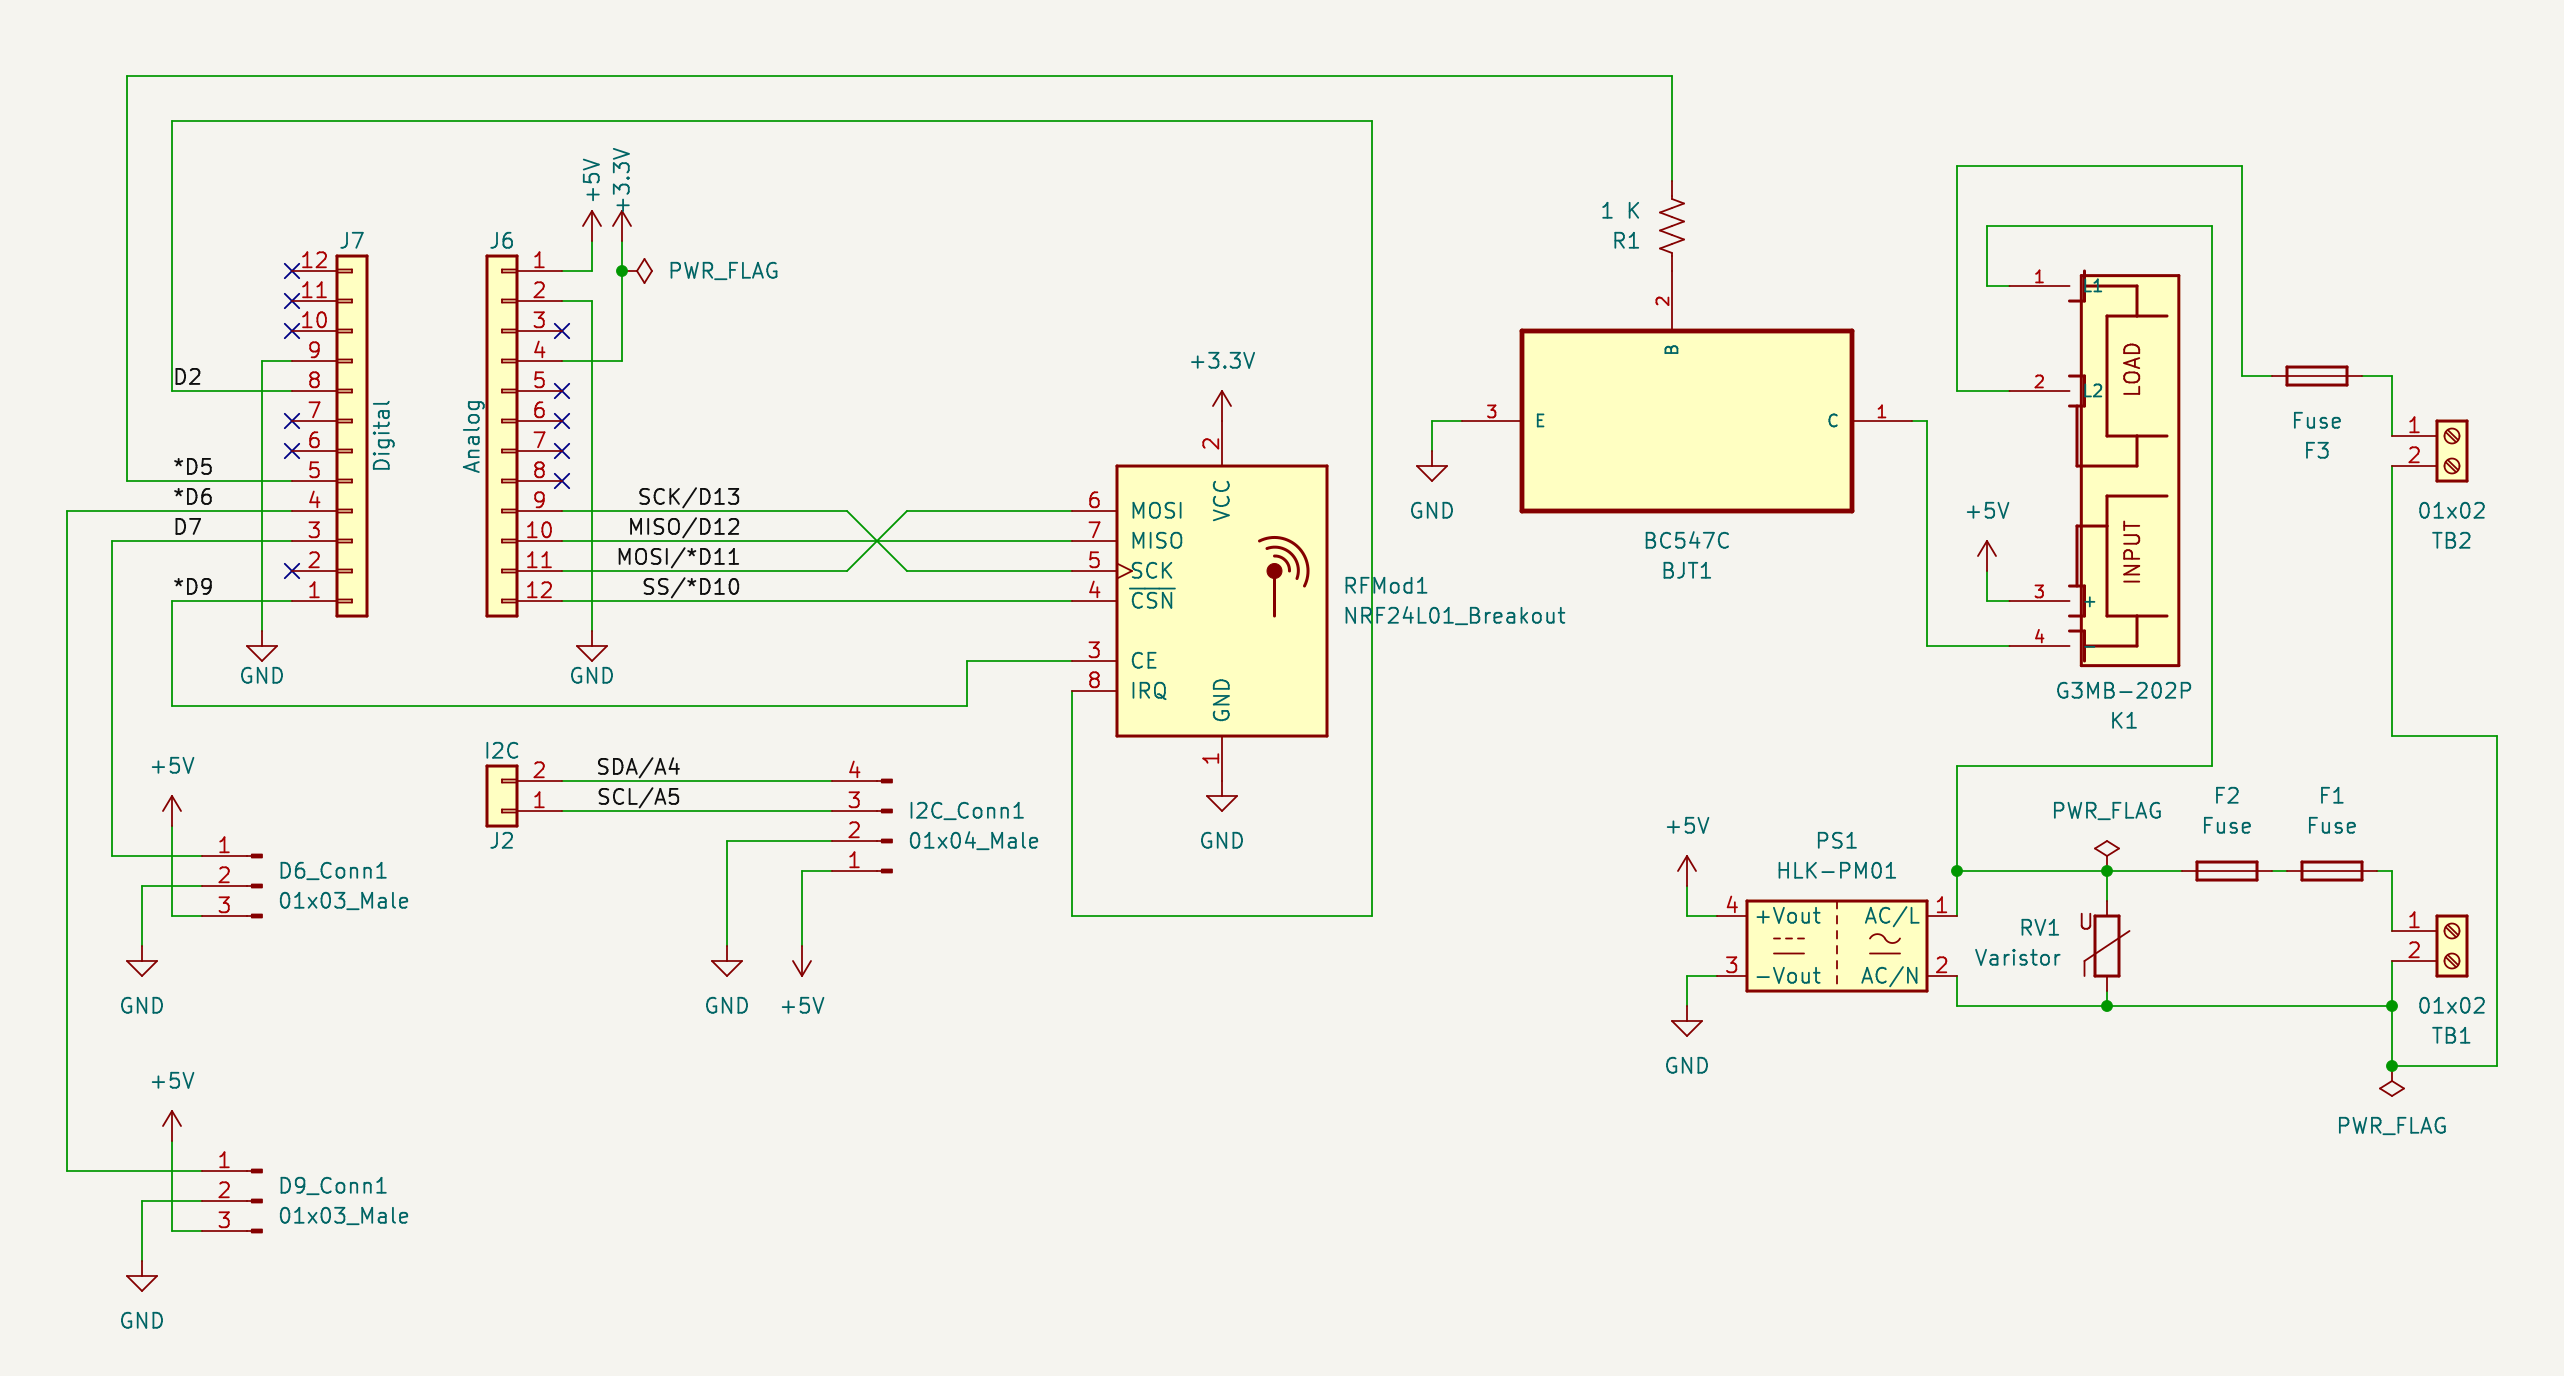
\includegraphics[width=\linewidth]{schematic-general.png}

\section{Huellas usadas}

%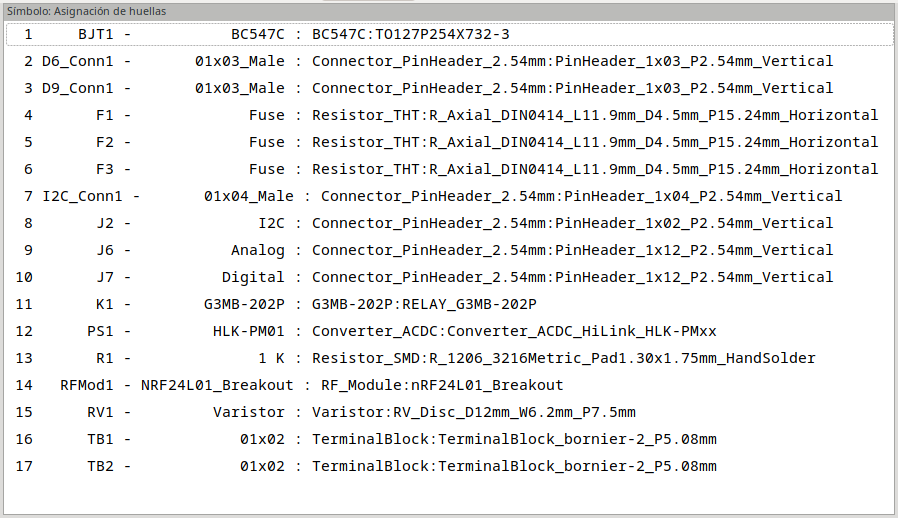
\includegraphics[width=\linewidth]{footprint-assignment.png}

% Indicar que la huella del BJT no es la estándar sino que es externa para
% facilitar su manipulación.

\section{Layout}

%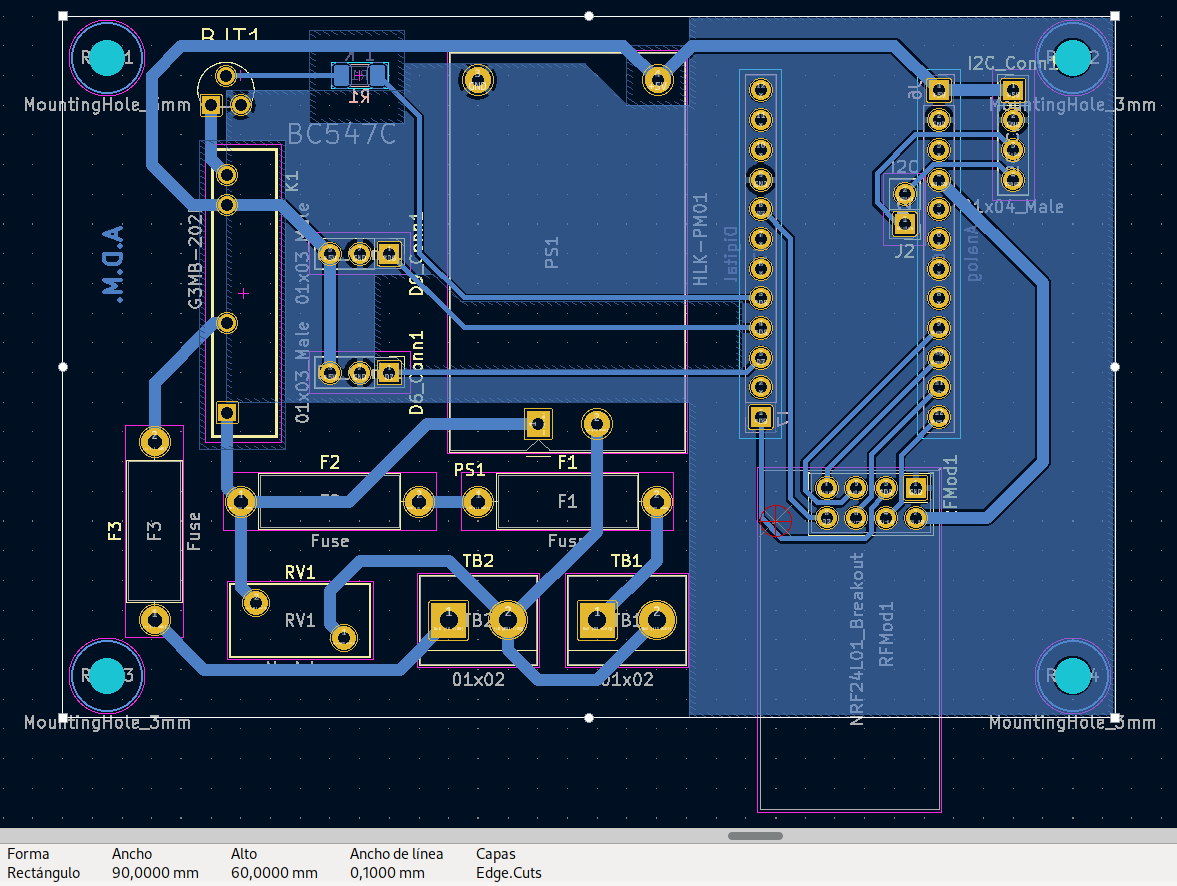
\includegraphics[width=\linewidth]{layout.png}

% Hay que cambiar el tamaño de los pads del varistor

\section{Generación de archivos Gerber}

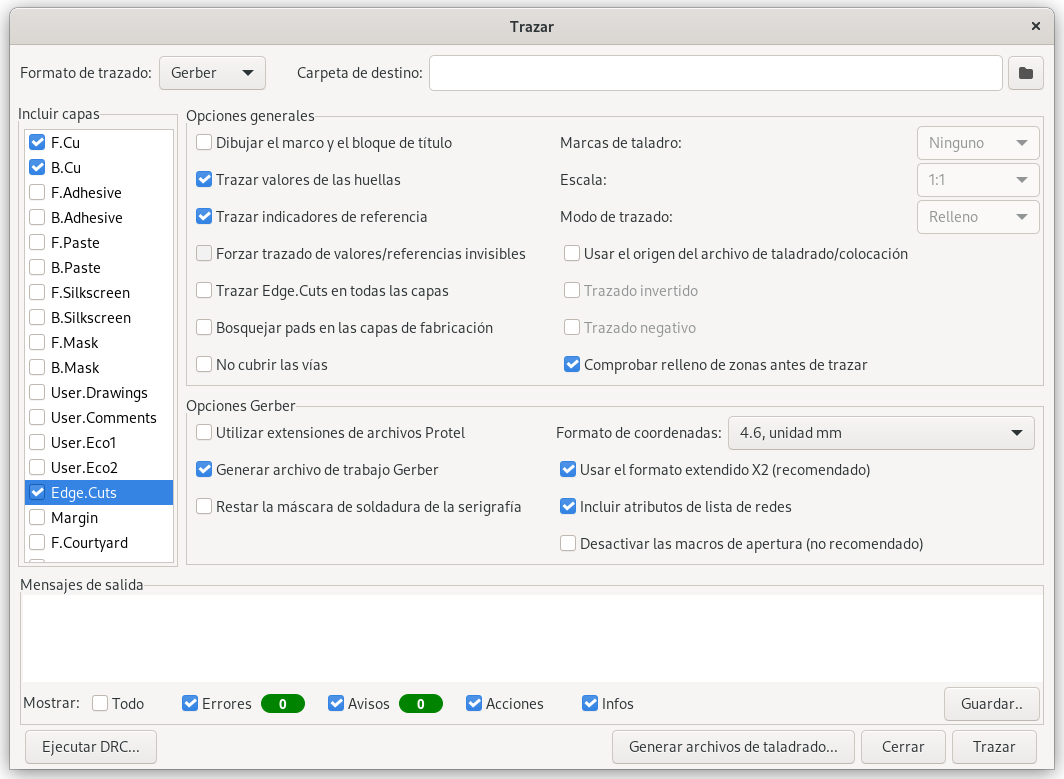
\includegraphics[width=\linewidth]{gerber-file-generation.png}

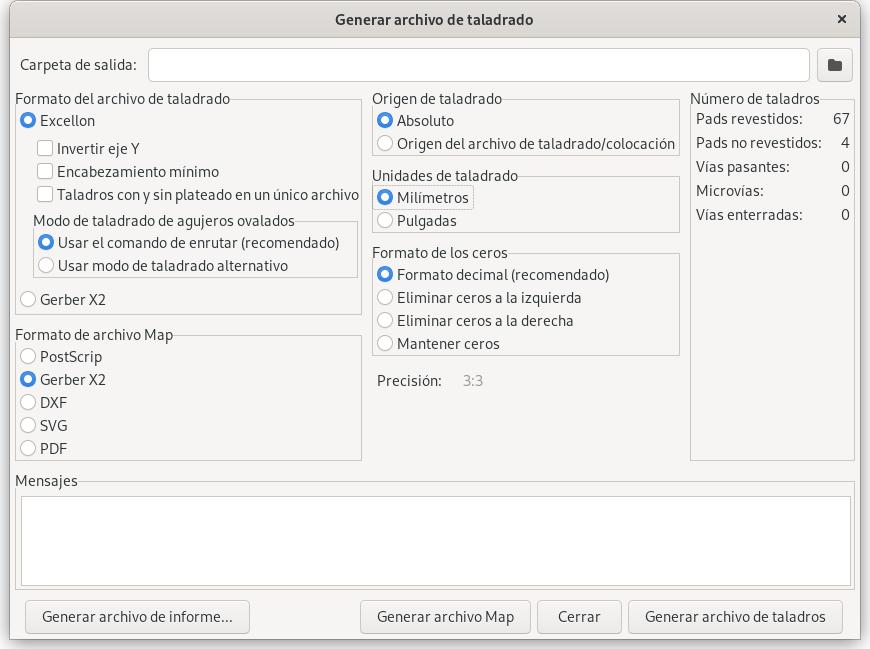
\includegraphics[width=\linewidth]{gerber-drilling-file-generation.png}

Es importante indicar que las unidades de taladrado sean en milímetros para que
los archivos resultantes sean utilizables por la máquina del departamento de la
asignatura, y así poder tener la placa PCB con las especificaciones correctas.

\section{Otros detalles}



\section{Resultado}

